% FLAGSHIP FIGURE: the runtime stack of RlmFrames IS the pushdown store. Each recursive
% subcall PUSHES a frame (depth_remaining strictly decreasing, budget telescoping); each
% stitched subresult POPS one. A run is well-nested iff every push is matched by a pop.
% Palette: frame/push=violet, pop=fuchsia, leaf=sky, accept=green.
\documentclass[border=12pt]{standalone}
\usepackage{tikz}
\usepackage{amsmath}
\usepackage{amssymb}
\usepackage{xcolor}
\usetikzlibrary{arrows.meta, positioning, fit, calc}
\definecolor{push}{HTML}{7C3AED}
\definecolor{pop}{HTML}{C026D3}
\definecolor{leaf}{HTML}{0284C7}
\definecolor{good}{HTML}{16A34A}
\definecolor{ink}{HTML}{1E293B}
\definecolor{slate}{HTML}{475569}
\begin{document}
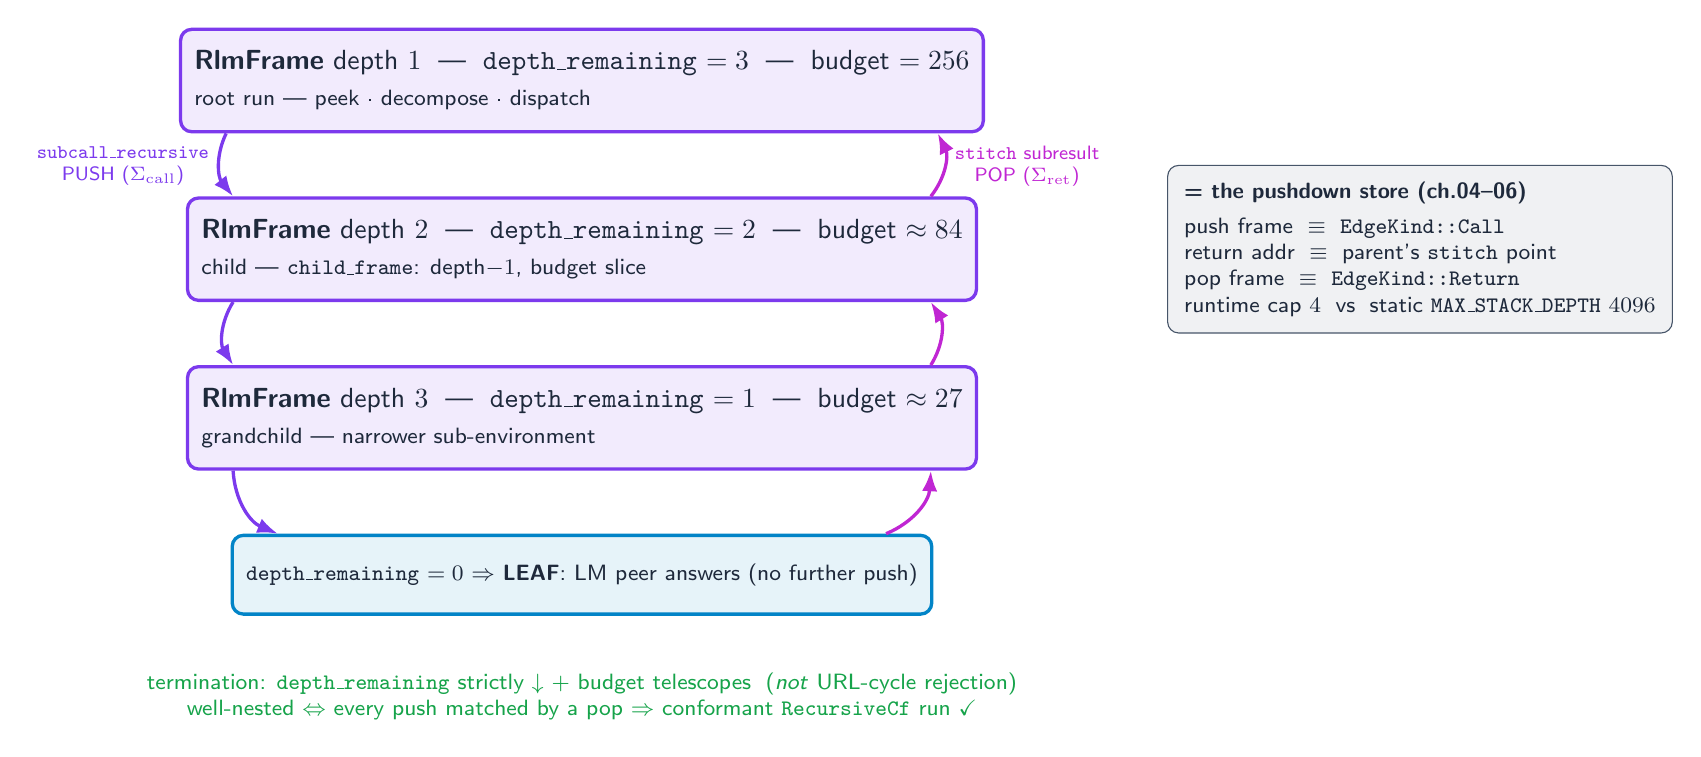
\begin{tikzpicture}[font=\sffamily, >={Latex[length=2.6mm]},
    frame/.style={draw=push, very thick, rounded corners, fill=push!10, text=ink,
                  minimum width=62mm, minimum height=13mm, align=left, inner sep=5pt}]

  % The frame stack (top = root, growing downward as we recurse).
  \node[frame] (f1) {\textbf{RlmFrame} depth $1$ \;|\; \texttt{depth\_remaining} $=3$ \;|\; budget $=256$\\[1pt]
    \footnotesize root run — peek · decompose · dispatch};
  \node[frame, below=8mm of f1] (f2) {\textbf{RlmFrame} depth $2$ \;|\; \texttt{depth\_remaining} $=2$ \;|\; budget $\approx 84$\\[1pt]
    \footnotesize child — \texttt{child\_frame}: depth$-1$, budget slice};
  \node[frame, below=8mm of f2] (f3) {\textbf{RlmFrame} depth $3$ \;|\; \texttt{depth\_remaining} $=1$ \;|\; budget $\approx 27$\\[1pt]
    \footnotesize grandchild — narrower sub-environment};
  \node[draw=leaf, very thick, rounded corners, fill=leaf!10, text=ink, minimum width=62mm,
        minimum height=10mm, align=left, inner sep=5pt, below=8mm of f3] (leaf)
    {\footnotesize \texttt{depth\_remaining} $=0$ $\Rightarrow$ \textbf{LEAF}: LM peer answers (no further push)};

  % Push arrows (left side, descending).
  \draw[->, push, very thick] ($(f1.south west)+(6mm,0)$) to[bend right=32]
        node[left, push, font=\sffamily\scriptsize, align=center]{\texttt{subcall\_recursive}\\PUSH ($\Sigma_{\mathrm{call}}$)} ($(f2.north west)+(6mm,0)$);
  \draw[->, push, very thick] ($(f2.south west)+(6mm,0)$) to[bend right=32] ($(f3.north west)+(6mm,0)$);
  \draw[->, push, very thick] ($(f3.south west)+(6mm,0)$) to[bend right=32] ($(leaf.north west)+(6mm,0)$);

  % Pop arrows (right side, ascending = stitch).
  \draw[->, pop, very thick] ($(leaf.north east)-(6mm,0)$) to[bend right=32] ($(f3.south east)-(6mm,0)$);
  \draw[->, pop, very thick] ($(f3.north east)-(6mm,0)$) to[bend right=32] ($(f2.south east)-(6mm,0)$);
  \draw[->, pop, very thick] ($(f2.north east)-(6mm,0)$) to[bend right=32]
        node[right, pop, font=\sffamily\scriptsize, align=center]{\texttt{stitch} subresult\\POP ($\Sigma_{\mathrm{ret}}$)} ($(f1.south east)-(6mm,0)$);

  % The correspondence panel.
  \node[draw=slate, rounded corners, fill=slate!8, text=ink, align=left, inner sep=6pt,
        right=24mm of f2, font=\sffamily\footnotesize] (corr)
    {\textbf{= the pushdown store (ch.04–06)}\\[3pt]
     push frame \;$\equiv$\; \texttt{EdgeKind::Call}\\
     return addr \;$\equiv$\; parent's \texttt{stitch} point\\
     pop frame \;$\equiv$\; \texttt{EdgeKind::Return}\\
     runtime cap $4$ \;vs\; static \texttt{MAX\_STACK\_DEPTH} $4096$};

  \node[good, font=\sffamily\footnotesize, align=center, below=6mm of leaf]
    {termination: \texttt{depth\_remaining} strictly $\downarrow$ + budget telescopes\; (\emph{not} URL-cycle rejection)\\
     well-nested $\Leftrightarrow$ every push matched by a pop $\Rightarrow$ conformant \texttt{RecursiveCf} run $\checkmark$};
\end{tikzpicture}
\end{document}
